\begin{figure}[h] 
\centering 
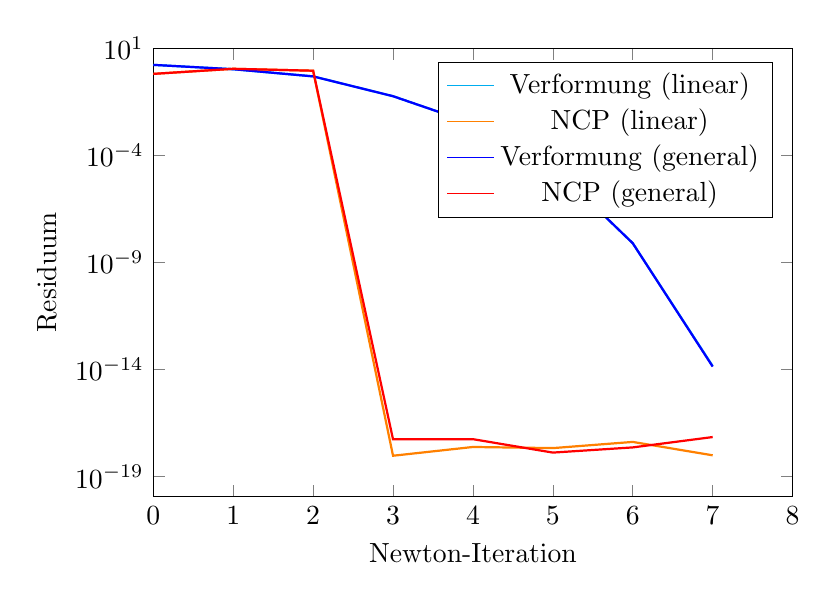
\begin{tikzpicture}[every plot/.append style={thick}] 
\begin{axis}[ 
label style={font=\normalsize}, 
xlabel={Newton-Iteration}, 
ylabel={Residuum}, 
xmin=0, xmax=8, 
ymode=log, 
ymin=0, ymax=10, 
width=0.8\textwidth, 
height=0.6\textwidth, 
legend pos=north east, 
legend style={cells={align=left}}, 
grid style=dashed, 
] 
\addplot[ 
color=cyan, 
] 
coordinates { 
(0, 1.66e+00)(1, 1.04e+00)(2, 4.82e-01)(3, 5.73e-02)(4, 3.00e-03)(5, 3.11e-05)(6, 7.89e-09)(7, 1.47e-14)}; 
\addlegendentry{Verformung (linear)} 
\addplot[ 
color=orange, 
] 
coordinates { 
(0, 6.31e-01)(1, 1.09e+00)(2, 8.86e-01)(3, 9.56e-19)(4, 2.45e-18)(5, 2.17e-18)(6, 4.22e-18)(7, 1.00e-18)}; 
\addlegendentry{NCP (linear)} 
\addplot[ 
color=blue, 
] 
coordinates { 
(0, 1.66e+00)(1, 1.04e+00)(2, 4.82e-01)(3, 5.73e-02)(4, 3.00e-03)(5, 3.11e-05)(6, 7.89e-09)(7, 1.38e-14)}; 
\addlegendentry{Verformung (general)} 
\addplot[ 
color=red, 
] 
coordinates { 
(0, 6.31e-01)(1, 1.09e+00)(2, 8.86e-01)(3, 5.57e-18)(4, 5.67e-18)(5, 1.34e-18)(6, 2.34e-18)(7, 7.12e-18)}; 
\addlegendentry{NCP (general)} 
\end{axis} 
\end{tikzpicture} 
\caption{Residuen des Stoffgesetzes 'St.Venant' mit Hinderniss 'Spitze' und 578 Freiheitsgraden für die Verschiebung.} 
\label{fiq:St.Venant_Spitze_level3} 
\end{figure} 
